Ebben a fejezetben átfogó képet adok az általam létrehozott helpdesk alkalmazásról. Az egyes komponensek részletes leírása \aref{ch:implementacio}. fejezetben található.

\section{Legfontosabb komponensek}

\begin{figure}[hbt] 
	\centering
	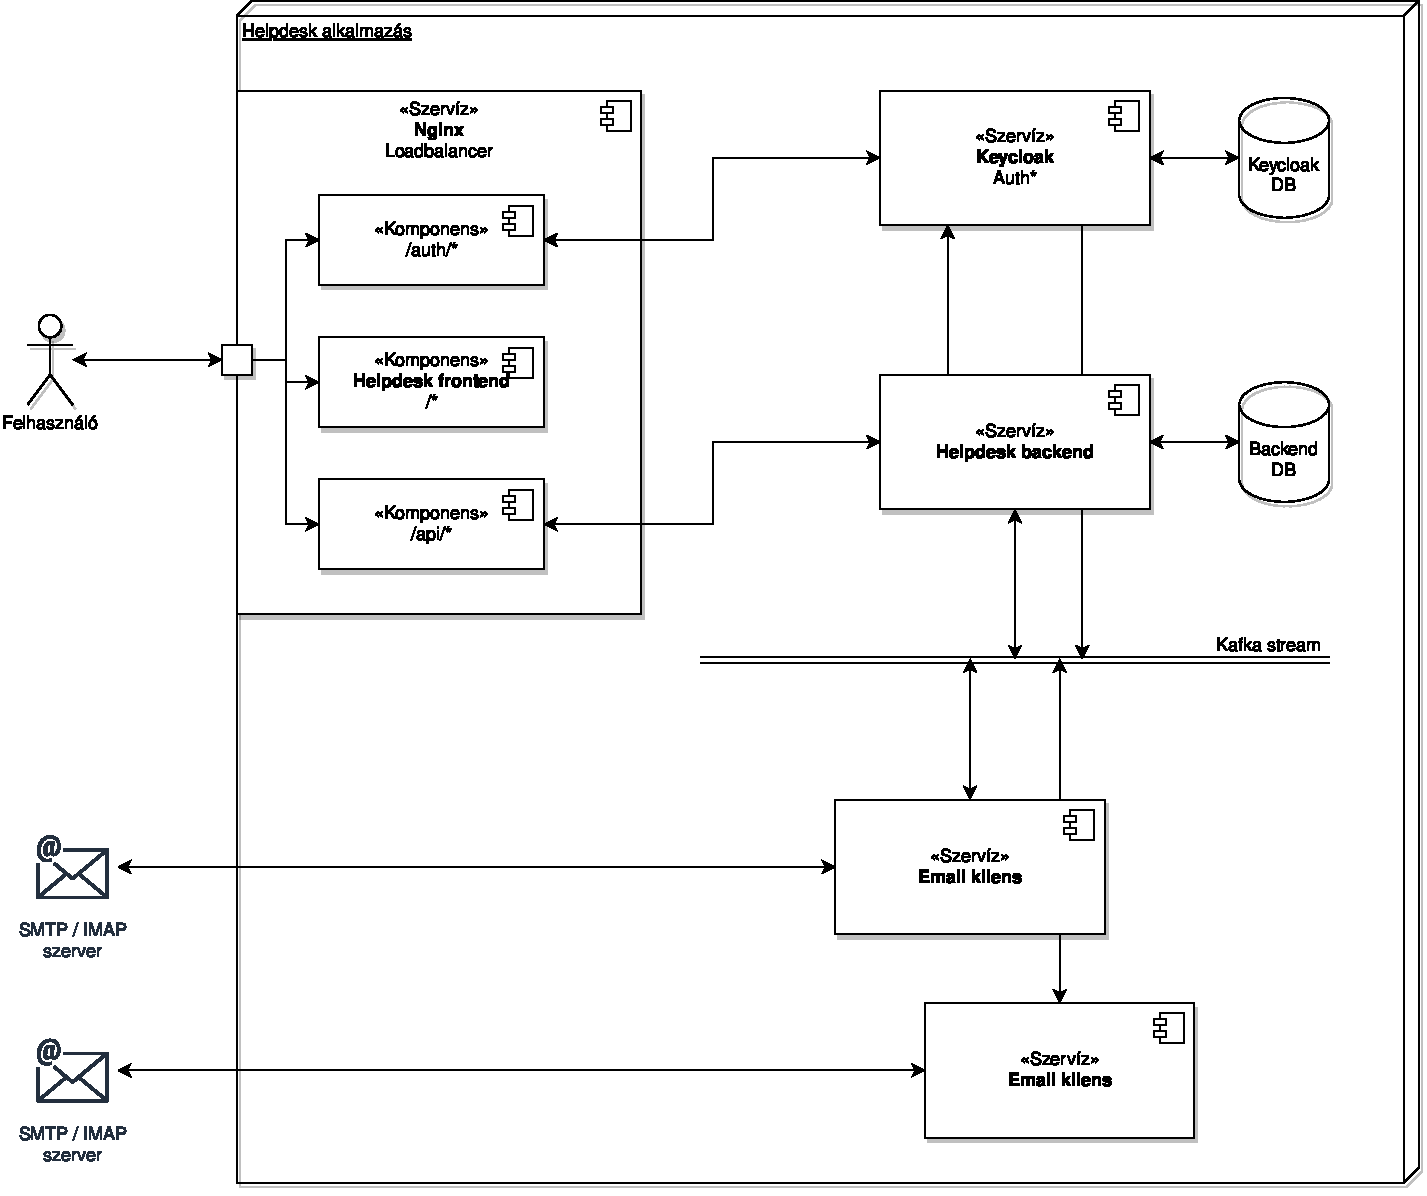
\includegraphics[width=0.87\textwidth]{komponens_diagram_drawio.pdf}
	\caption{A legfontosabb komponensek}
	\label{fig:komponens_diagram}
	\floatfoot{Forrás: saját ábra}
\end{figure}

\Aref{fig:komponens_diagram}. ábrán a legfontosabb szolgáltatásokat gyűjtöttem össze. Az üzleti funkcionalitás megvalósulása az itt bemutatott komponensek összehangolt munkáján keresztül valósul meg.


\begin{itemize}
	\item A felhasználó az nginx-en (\ref{sec:nginx} pont) keresztül éri el a helpdesk alkalmazást. Az ő perspektívájából nem látszik az alkalmazás réteges, széttagolt felépítése.
	\item Az nginx az üzenet URL-je alapján dönti el, hogy melyik kérést, melyik szolgáltatás szolgáljon ki.
	\item Az e-mail kliens és a heldpesk backend kafka streamen keresztül éri el egymást. Közvetlenül nem kommunikálnak.
	\item Az e-mail kliensek kezelik az e-mail szerverekkel való adatcserét. Az e-mailek fogadásáért és küldéséért felelősek.
	\item A Keycloak szolgáltatás adatot küld a kafka streamen keresztül, amit a helpdesk backend fogad.
\end{itemize}


\section{Adatbázis UML diagram}\label{sec:felepites_adatbazis}
A helpdesk backend adatbázis legfontosabb tábláit \aref{fig:basic_database_uml}. ábra tartalmazza. Az ábrán nem szerepelnek az audit és a Liquibase által használt táblák~(\ref{sec:adatbazis} pont), azokat --~az összes többi táblával együtt~-- \aref{ch:bemutatas}. fejezetben található \ref{fig:extended_database_uml}. ábra tartalmazza.
 
 \begin{figure}[hbt] 
 	\centering
 	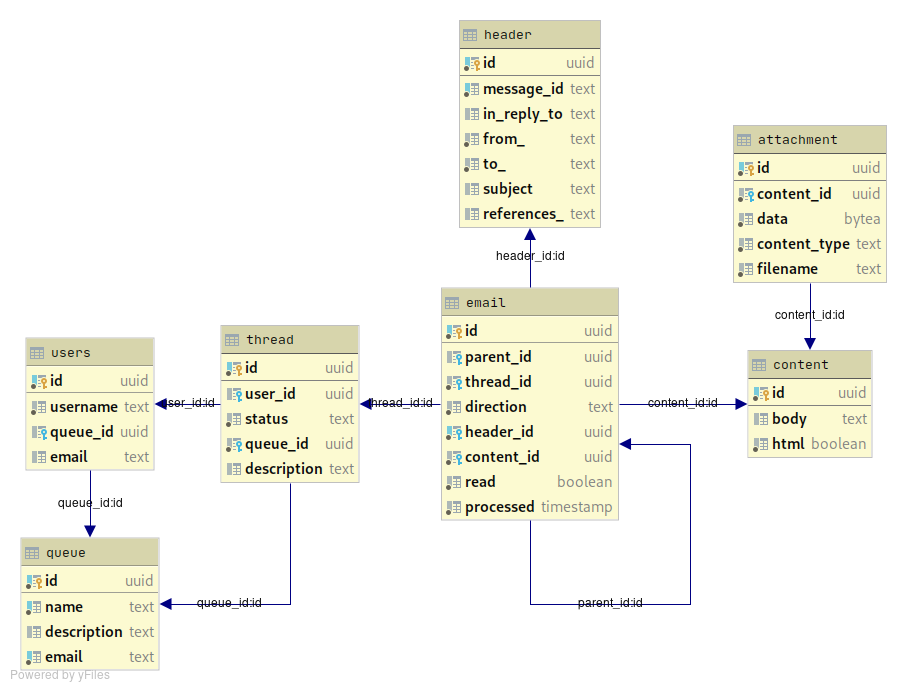
\includegraphics[width=0.85\textwidth]{basic_database_uml.png}
 	\caption{A backend legfontosabb adatbázistáblái}
 	\label{fig:basic_database_uml}
 	\floatfoot{Forrás: saját ábra}
 \end{figure}


\Aref{fig:basic_database_uml}. ábrán megjelenített adatszerkezetről elmondható, hogy:
\begin{itemize}
	\item egy felhasználó (\texttt{users}~tábla) pontosan egy sorhoz (\texttt{queue}~tábla) tartozik, és több e-mail szállal rendelkezhet;
	
	\item egy e-mail szál (\texttt{threads}~tábla) potosan egy sorhoz tartozik, és csupán egy felhasználóhoz tartozhat. Egy e-mail szálhoz legalább egy e-mail tartozik;
	
	\item egy e-mailnek (\texttt{email}~tábla) pontosan egy fejléce (\texttt{header}~tábla) és egy tartalma (\texttt{content}~tábla) van, valamint pontosan egy  e-mail szálhoz tartozik. Ezen kívül, minden e-mail legfeljebb egy szülő e-mail alá tartozhat;

	\item egy e-mail tartalomnak (\texttt{content}~tábla) nulla vagy több csatolmánya (\texttt{attachment}~tábla) lehet.
\end{itemize}

Az adatbázis hármas normálformában van, mert az entitások minden tulajdonsága csak az entitás teljes kulcsától függ, és a kulcson kívül semmilyen más tulajdonságától nem függ.



\section{E-mail fogadásának és küldésének folyamata}
A könnyebb átláthatóság érdekében, a folyamatokat egy e-mail szemszögéből mutatom be \aref{fig:path_of_an_email}. ábrán. Az e-mail fogadása az alábbi felsorolás által leírt folyamat szerint történik.
\begin{enumerate}
	\item Az e-mail kliens IMAP protokollon keresztül megkapja az új e-mailt.
	\item Az e-mail kliens a bejövő e-mailt egy kafka üzenetként teszi közzé a bejövő e-mailek kafka \emph{topicban}.
	\item A bejövő e-mailek \emph{topic}ra feliratkozott helpdesk backend megkapja a kafka üzenetet.
	\item A helpdesk backend eltárolja az új üzenetet az adatbázisban
	\item A felhasználó a frontend segítségével lekérdezi az újonnan beérkezett e-maileket.
	\item A helpdesk backend a kérésre elküldi az újonnan fogadott e-mailt.
\end{enumerate}

\bigskip
Az e-mail küldése pedig az alábbi felsorolás szerint hajtódik végre.
\begin{enumerate}
	\item A felhasználó az új e-mail elolvasása után a frontend segítségével megírja a választ.
	\item A felhasználó elküldi a választ a helpdesk backendnek.
	\item A helpdesk backend eltárolja az adatbázisba az új e-mailt, majd az e-mail szálnak megfelelő kimenő e-mail \emph{topic}ba közzéteszi az új üzenetet.
	\item Az e-mail cím specifikus kimenő e-mailek \emph{topic}ra feliratkozott e-mail kliens megkapja a kafka üzenetet.
	\item Az e-mail kliens SMTP protokollon keresztül elküldi az új e-mailt.
\end{enumerate}


\begin{figure}[hbt] 
	\centering
	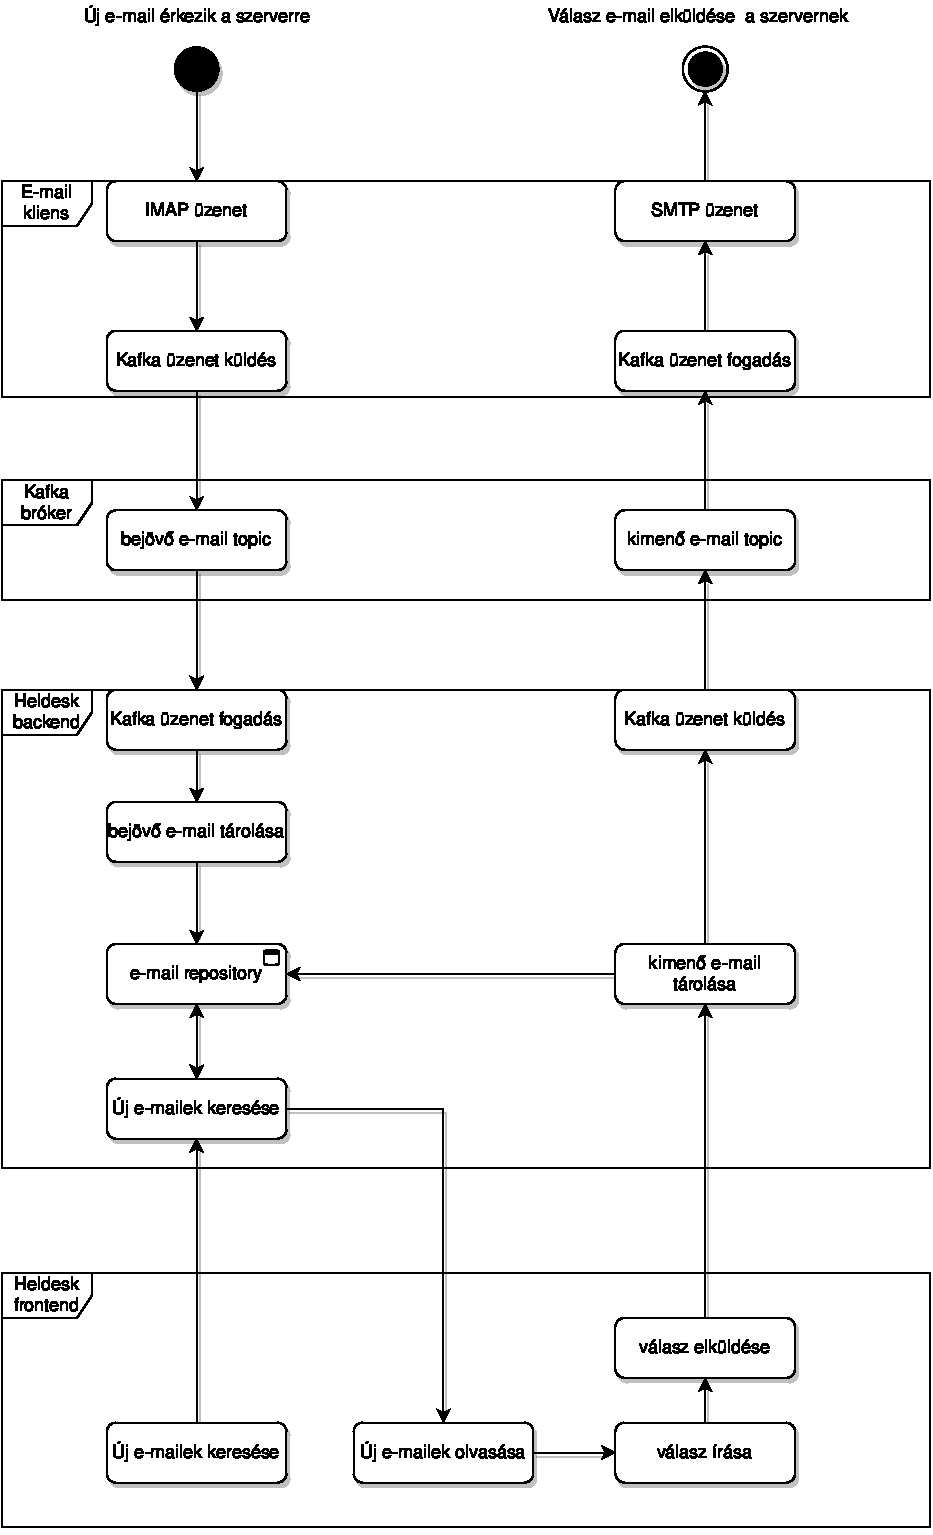
\includegraphics[width=0.7\textwidth]{path_of_an_email_drawio.pdf}
	\caption{A bejövő és kimenő e-mail útja}
	\label{fig:path_of_an_email}
	\floatfoot{Forrás: saját ábra}
\end{figure}
